\section{Diseño}
Si se parte del circuito típico para un resonador LC paralelo, el mismo resonará a una frecuencia $f_0$ dada por

$$
f_0 = \frac{1}{2\pi\sqrt{LC}}
$$

\begin{figure}[H]
    \centering
    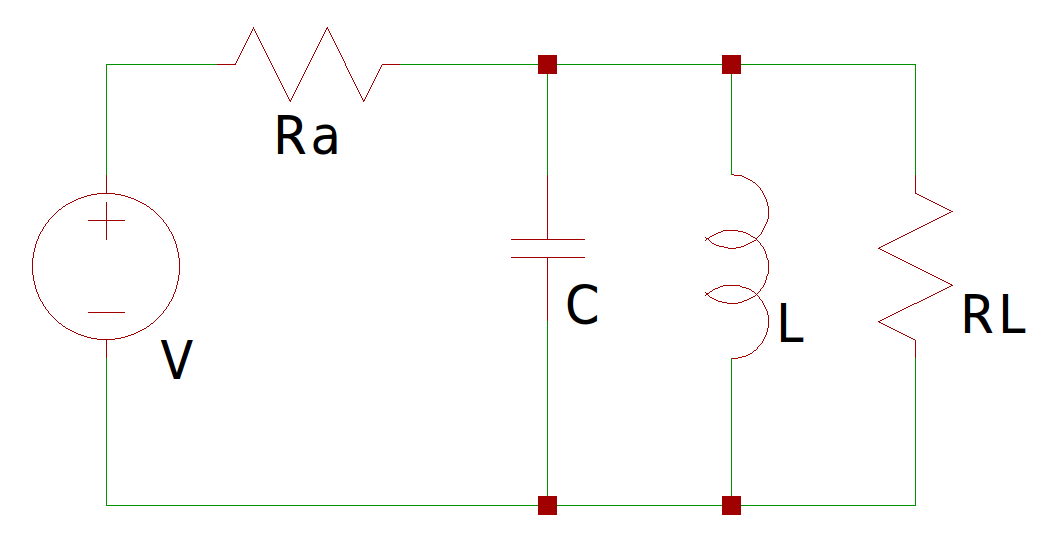
\includegraphics[width=0.5\linewidth]{fig/lcparalelo.png}
    \caption{circuito LC paralelo}
    \label{fig:enter-label}
\end{figure}

Además

$$
Q = \frac{f_0}{BW} = \frac{R_T}{X_L}   
$$

Donde $BW$ representa el ancho de banda del circuito. La resistencia total $R_T$ del circuito esta definida por la impedancia de entrada $R_a$, la impedancia de salida $R_L$ y la resistencia de pérdida del inductor $R_P$. Para este análisis se desprecia la pérdida en los capacitores. En este circuito, no podemos elegir el ancho de banda, puesto que el mismo depende de las impedancias de entrada y salida.

$$
R_T = R_a//R_p//R_L
$$

Para poder elegir de manera independiente el ancho de banda y lograr adaptar impedancias de entrada y salida, se debe de adoptar ciertas modificaciones en el circuito. Si se divide el capacitor $C$ en cuatro capacitores, se tiene el siguiente circuito.

\begin{figure}[H]
    \centering
    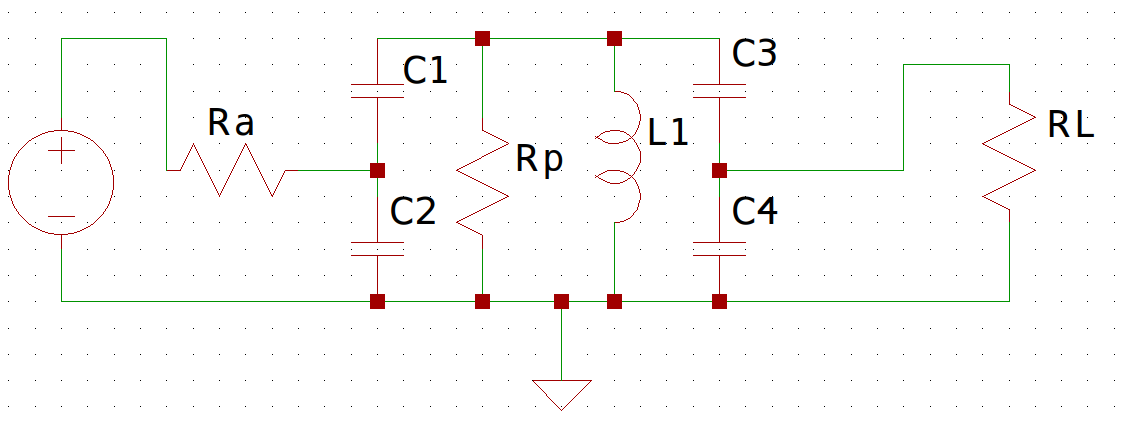
\includegraphics[width=0.5\linewidth]{fig/circuito.png}
    \caption{acoplador}
    \label{fig:enter-label}
\end{figure}

Para no alterar el la frecuencia de resonancia $f_0$ del circuito, se debe procurar que la capacidad equivalente se mantenga igual, es decir

$$
C = \frac{1}{1/C_1+1/C_2} + \frac{1}{1/C_3+1/C_4}
$$

De esta forma, la impedancia de entrada y de salida son adaptadas por un factor de transformación, dados por los pares de capacitores $C_1,C_2$ y $C_3,C_4$, para $R_a$ y $R_L$ respectivamente. 

\subsection{Transformador Capacitivo}

Si se realiza el analisis de la impedancia en una de las ramas, se tiene que la admitancia equivalente $Y_e$ esta dada por

\begin{figure}
    \centering
    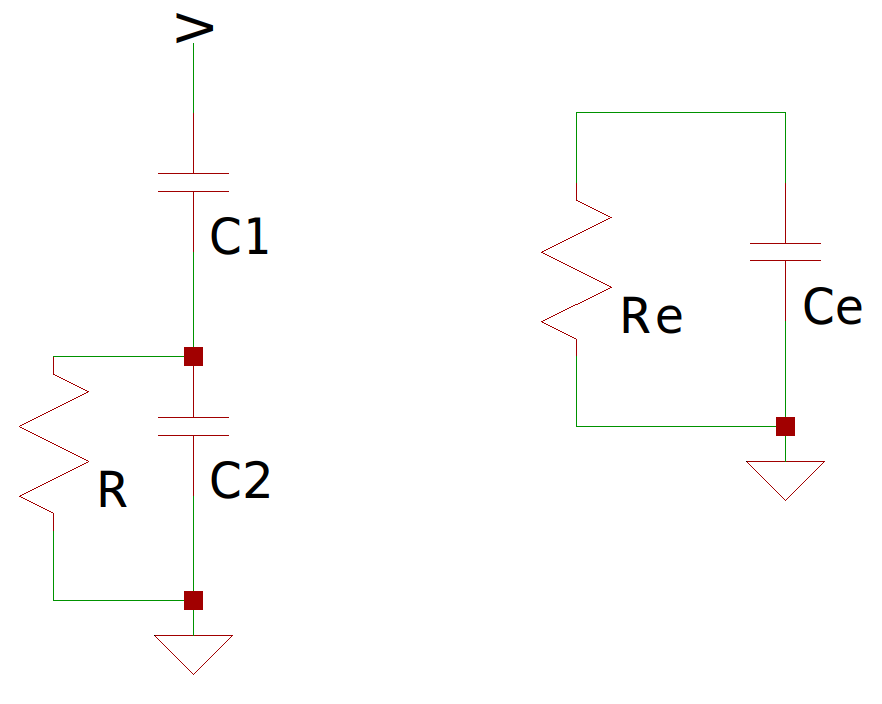
\includegraphics[width=0.5\linewidth]{fig/divcap.png}
    \caption{circuito equivalente del divisor capacitivo}
    \label{fig:enter-label}
\end{figure}

$$
Y_{s1} = \frac{1}{R_e}+\frac{1}{XC_2} 
$$
$$
Y_e = \frac{Y_{s1}*1/XC_1}{Y_{s1}+1/XC_1}
$$
$$
Y_e = \frac{1+jwC_2R}{1+jw(C_1+C_2)R}jwC_1
$$

Multiplicando por el conjugado y reordenando, obtenemos
$$
Y_e = \frac{1-jw(C_1+C_2)R+jwC_2R+w^2C_2+R^2(C_1+C_2)}{1+w^2(C_1+C_2)R^2}jwC_1
$$

$$
Y_e = \frac{w^2C_1^2R+jwC_1[1+w^2C_2R^2(C_1+C_2)]}{1+w^2R^2(C_1+C_2)^2}
$$

Pero si tenemos que $1<<w^2R^2(C_1+C_2)^2$ y $1<<1+w^2C_2R^2(C_1+C_2)]$ por ser $w$ muy grande

$$
Y_e = \frac{w^2C_1^2R+jw^3C_1C_2R^2(C_1+C_2)}{w^2R^2(C_1+C_2)^2}
$$

Si separamos los terminos reales de los terminos complejos, obtenemos

$$
Y_e = \frac{C_1^2}{(C_1+C_2)^2}*\frac{1}{R}+jw*\frac{C_1C_2}{C_1+C_2}
$$

Entonces

$$R_e = R\frac{C1+C2}{C1}^2=R*(1+\frac{C_2}{C_1})^2$$

$$
C_e = \frac{C_1*C_2}{C_1+C_2}
$$

Por lo tanto, podemos reescribir las impedancias equivalentes $R'_a$ y $R_L'$ como

$$
R_a' = \left( 1 + \frac{C_2}{C_1} \right)^2 R_a \\
$$
$$
R_L' = \left( 1 + \frac{C_3}{C_4} \right)^2 R_L
$$

A partir de las impedancias equivalentes sobre $L$, ahora $R_T$ está dada por

$$
R_T = R_a'//R_p'//R_L
$$

\subsection{Selección de $L$}

Puesto que existen infinitos pares de $L$ y $C$ que satisfagan la condición de $f_0$, se deben plantear ciertos criterios a la hora de elegir los valores correspondientes. Para una determinada $f_0$, utilizar capacidades muy grandes resulta en inductores muy pequeños y viceversa. Se plantea conformar iterativamente una gran cantidad de pares LC para satisfacer las especificaciones de diseño. El cálculo de $L$ se realizó asumiendo ciertos parámetros físicos, como la sección del cobre y el paso de las espiras.

Partiendo de los requerimientos de diseño

\begin{enumerate}
    \item $f_0 = 18 MHz$
    \item $BW = 1MHz$
    \item $Z_{in}=50\Omega$
    \item $Z_{Out} = 1K\Omega$
\end{enumerate}

Se calcularon de forma tabulada varios pares LC. Los mismos se encuentran detallados en el archivo de \textit{jupyter notebook} llamado \textit{tabla.ipynb}.

En el código, se definen los siguientes parámetros iniciales:
\begin{itemize}
    \item \( f_o = 18 \) MHz: Frecuencia de operación.
    \item \( d = 0.15 \) cm: Diámetro del conductor.
    \item \( D = 1.65 \) cm: Diámetro del núcleo.
    \item \( s = d \): Separación entre espiras (igual al diámetro del conductor).
    \item \( p = s + d \): Paso de la espira.
    \item \( N_s = \frac{1}{s + d} \): Número de vueltas por cm.
    \item \( Q_c = 10 \): Factor de calidad de acoplamiento.
    \item \( R_g = 50 \) \( \Omega \): Resistencia del generador.
    \item \( R_l = 1000 \) \( \Omega \): Resistencia de carga.
\end{itemize}

Se ejecuta un bucle que varía la capacitancia en pasos de 10 pF, y para cada valor se obtiene $K$ y $l/D$ a partir de una interpolación de la curva del factor de Nagaoka tabulado. El número de vueltas del inductor de núcleo de aire es calculado a partir de $Ns$ y $l$.

\begin{figure}[H]
    \centering
    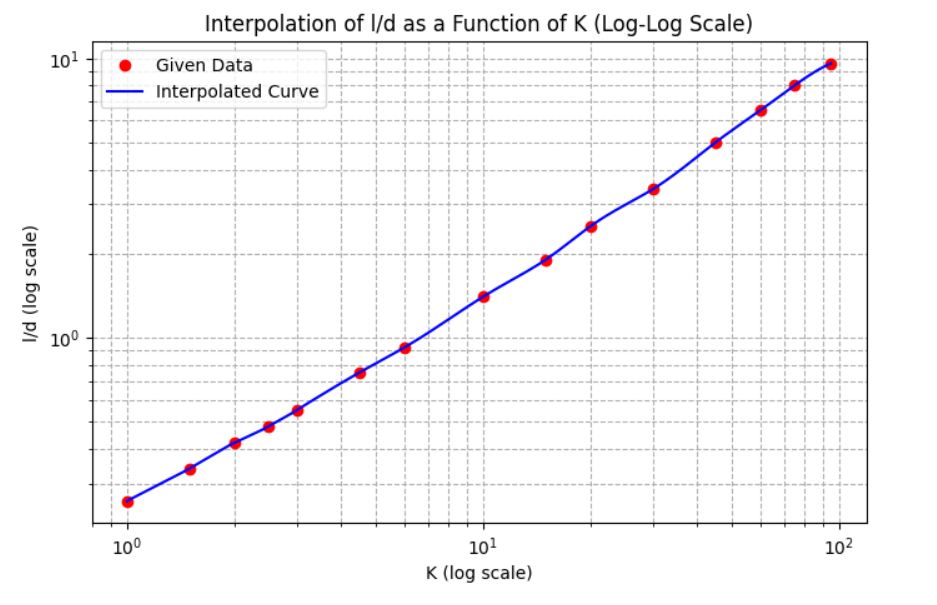
\includegraphics[width=0.5\linewidth]{fig/interpolacion.png}
    \caption{interpolación de los valores tabulados del factor de Nagaoka}
    \label{fig:enter-label}
\end{figure}

\subsection{Selección de Capacitores}

Una vez obtenidos los parámetros del inductor, tambien se calcula la combinación necesaria de capacitores $C_1$, $C_2$, $C_3$ y $C_4$ a partir de la resistencia de pérdida del inductor, la impedancia de entrada y salida y el ancho de banda.
$$
    C_2 = \frac{C}{2} \sqrt{\frac{R_{ap}}{R_g}}
$$
$$
    C_1 = \frac{C}{2} \times \frac{C_2}{C_2 - C/2} 
$$
$$
    C_4 = \frac{C}{2} \sqrt{\frac{R_{Lp}}{R_l}} 
$$
$$
C_3 = \frac{C}{2} \times \frac{C_4}{C_4 - C/2} 
$$

Los capacitores utilizados deben tener valores realizables, esto quiere decir que el inductor se descarta si sus parámetros generan valores de capacitores negativos o demasiado pequeños.

\subsection{Parámetros Finales}
Los valores finales para los componentes a utilizar son:
\[
\begin{array}{|c|c|c|}
\hline
\textbf{Parameter} & \textbf{Value} & \textbf{Unit} \\
\hline
C & 150.000 & \text{pF} \\
L & 521.200 & \text{nH} \\
N_s & 3.333 & \text{vueltas/cm} \\
K & 10.442 & \text{-} \\
l_d & 1.4478908999912352 & \text{} \\
l & 2.389 & \text{cm} \\
N & 7.963 & \text{vueltas} \\
Q & 449.753 & \text{-} \\
X_L & 58.946 & \Omega \\
R_p & 26.511 & K\Omega \\
R_t & 589.463 & \Omega \\
R_{ap} & 1.179 & K\Omega \\
R_{Lp} & 1.234 & K\Omega \\
C_1 & 94.451 & \text{pF} \\
C_2 & 364.183 & \text{pF} \\
C_3 & 752.132 & \text{pF} \\
C_4 & 83.307 & \text{pF} \\
C_t & 150.000 & \text{pF} \\
\hline
\end{array}
\]